% !TEX root = demo.tex
\section{Introduction}\label{sec:intro}

\begin{figure}[t]
\centering
\vspace{-0.5cm}
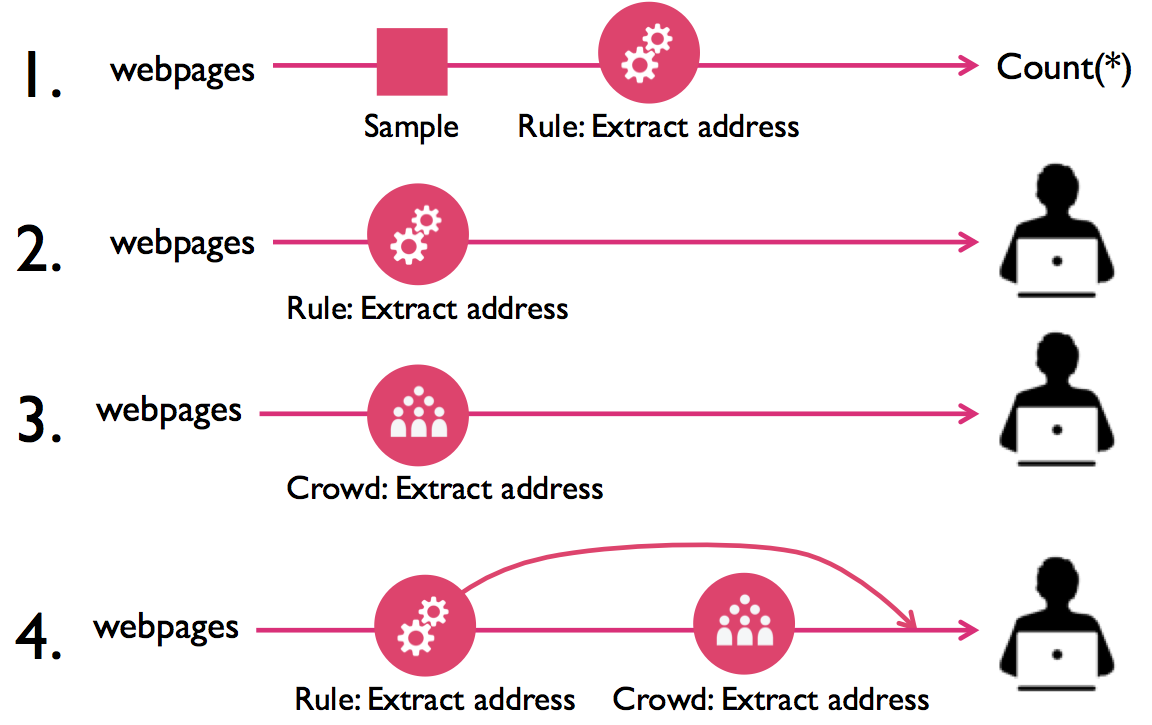
\includegraphics[width = .4\textwidth]{figs/lifecycle.png}
\vspace{-0.2cm}
\caption{Example iterations on the design of the portion of a cleaning plan that extracts restaurant addresses from their unstructured webpages.  
1) An exploratory plan that uses a sample to evaluate a simple address extraction method.
2) A plan that applies the method to the entire dataset. The quality is unsatisfactory. 
3) An alternate plan that uses manual crowd extraction. The quality is now high, but the crowd-based extractor is slow. 
4) A hybrid plan that sends only difficult webpages to the crowd, maximizing accuracy without sacrificing latency.}
\label{fig:ex-plan}
\vspace{-0.6cm}
\end{figure}
% why feedback loops exist/are important (cite Joe’s shit in the past 3 years, blinkdb, etc.). highlight domain specificity. Large variety of data cleaning tasks

%
% General comment that data cleaning is important:
%
The prevalence of dirty data presents a fundamental obstacle to modern data-driven applications, since 
blindly using results that are derived from dirty data can lead to hidden, yet significant errors.
Analysts report spending upwards of 80\% of their time on problems in data cleaning \cite{kandel2012} including 
error diagnosis, instance-specific cleaning scripts, and managing large data ingest pipelines.
The underlying problem is that data cleaning is often specific to the domain, dataset, and eventual analysis,
leading to a breadth of possible errors that are manifest in the data and a variety of options to clean it.
The user must go through the cleaning process with little or no guidance, deciding for each of her data sources what to extract, how to clean it, and whether that cleaning will significantly change results.

Figure~\ref{fig:ex-plan} shows a common progression for the development of a data cleaning operator, in this case the extraction of a restaurant's address from its unstructured webpage.
Though this operation can easily be represented at a \textit{logical} level by its inputs and outputs, there is a huge space of possible \textit{physical} implementations of the logical operator. 
For example, extraction could be rule-based, rely on structured learning, ask crowd workers to extract the desired data fields, or some combination of all three.
Even after selecting (say) a crowd-based operator, many parameters might influence the quality of the output data or the speed and cost of cleaning it: the number of crowd workers who vote on the extraction for a given webpage, the amount each worker is paid, etc.
A priori, a data analyst has little intuition for what physical plan will be optimal in this large space.

In practice, she will likely start by sampling the data, applying a simple method such as a rule-based approach, and querying the output to get a sense of the method's effectiveness (Figure~\ref{fig:ex-plan}.1).
If the approach seems promising, she will apply the method to the entire dataset (Figure~\ref{fig:ex-plan}.2).
However, the first approach tried seldom yields the desired accuracy, so the data analyst might have to experiment with other physical operators, for example a crowd operator that uses human workers to manually perform the extraction (Figure~\ref{fig:ex-plan}.3).
Though such adjustments might improve accuracy, using the crowd to process every webpage is prohibitively slow.
To achieved the desired accuracy without sacrificing speed, the data analyst now must experiment with hybrid physical implementations (Figure~\ref{fig:ex-plan}.4).
Though this iterative design process eventually produces a satisfactory physical implementation of the extraction logical operator, to prepare the restaurant dataset for analysis, our analyst must implement and chain together several logical operators, e.g. eliminating duplicate restaurants from the dataset or canonicalizing categorical variables such as cuisine type.
Without a general, scalable, and interactive system that supports rapid iteration on candidate cleaning plans, analysts have to manually construct a physical plan for each logical operator, requiring significant manual coding and parameter optimization.

%The prevalance of data cleaning systems in both the research and industrial communities --
%Corleone does blah, XXX addresses blah. Nadeef does blah -- speak to the importance of a
%data cleaning framework as part of the modern big data ecosystems. \ewu{include open access of data in argument?} \jn{We also need to take a look at data cleaning systems in industry. }


% why existing systems suck aka related work
% 1. have slow feedback loops (dataset-dependence, …)
% 2. solve very specific data-cleaning tasks
Since the beginning of data management, systems have been explored by both the research and industrial communities to improve data cleaning efficiency and quality.
However, no existing systems address the end-to-end iterative data cleaning process described above.
Extract-transform-load (ETL) systems~\cite{informatica,talend,apachefalcon} require developers to manually write data cleaning rules and execute them as long batch jobs, 
and constraint-driven tools allow analysts to define ``data quality rules" and automatically propose corrections to maximally satisfy these rules \cite{DBLP:conf/sigmod/DallachiesaEEEIOT13}.
Unfortunately, neither provide the opportunity for iteration or user feedback, inhibiting the user's ability to rapidly prototype different data cleaning solutions.
Projects such as Wrangler~\cite{wrangler,trifacta} and OpenRefine~\cite{openrefine} support iteration with spreadsheet-style interfaces that enable the user to compose data cleaning sequences by directly manipulating a sample of the data and applying these sequences to the full dataset.
However, they are limited to specific cleaning tasks such as simple text transformations, do not support crowd-based processing at scale, and cannot incorporate user feedback to optimize the physical implementation of the data cleaning sequences.
Crowd-based~\cite{gokhale2014corleone,stonebraker2013data} systems have been proposed to relieve the data cleaning analyst of the burden of rule specification or manual cleaning, but are usually very task specific (e.g., de-duplication~\cite{gokhale2014corleone,park2014crowdfill,eracer,chen2014integrating}) and require analysts to awkwardly chain systems together to execute the entire cleaning workflow, preventing end-to-end optimization of the entire plan.
These existing limitations suggest the need for a system that is general enough to adapt to a wide range of data cleaning applications, scales to large datasets, and natively supports fast-feedback interactions to enable rapid data cleaning iteration.

In this paper, we introduce \sys, a system designed to support the iterative development and optimization of data cleaning plans end to end.
\sys allows users to specify declarative data cleaning plans composed of rule-based, learning-based, or crowd-based operators, then enabling rapid iteration on plans with cost-aware recommendations for improving the accuracy or latency of a plan by swapping in new physical operators or modifying their parameters.
Early, exploratory plans are supported with sampling and approximate query processing techniques~\cite{wang1999sample}.
\sys additionally provides users with the opportunity to provide ground-truth feedback after each logical operator in the plan to improve recommendations, and supports adjusting in-flight plans efficiently using caching and tuple lineage.

Supporting these capabilities requires a combination of careful engineering 
as well as tackling several research challenges:

\squishlist
\item \textbf{Sampling}: We provide sampling as a first-class logical operator for data cleaning plans that tolerate approximation, and use it to speed up iteration on early-stage plans.

\item \textbf{Recommendation}: We leverage interactive user feedback to recommend cost-aware changes to in-flight cleaning plans that allow users to trade off accuracy and latency, and provide efficient mechanisms for implementing recommended changes without re-executing the plan on already cleaned tuples.

\item \textbf{Crowd Latency}: We leverage techniques for straggler mitigation~\cite{venkataraman2014power} and model crowd worker speed and accuracy to reduce the (often rate-limiting) latency of crowd data cleaning, consistently retrieving results in seconds rather than hours.
\squishend

In our demonstration, we will run an entity resolution plan on two restaurant datasets, and
show how \sys can be used to 1) specify and execute a data cleaning plan using our domain specific
language, 2) quickly clean a sample to characterize how a plan is performing, 
3) observe that cleaning plans are not necessarily optimal across datasets, and 
4) incrementally refine the plan to fit a new dataset by changing an operator's parameter (e.g., similarity threshold)
or its physical implementation.
The fourth interaction lets the participants inspect the effects of different physical plans.
Users can then execute a plan over a live crowd that uses the audience as workers, or a simulated crowd
that uses pre-collected crowd responses. The dashboard (Figure~\ref{screenshot-rec}) also provides a live inspection
interface to view the status of the cleaning plan as it executes.

\vspace{-0.2cm}
%Our contributions/requirements
%different ways to tighten the feedback loop:
%end-to-end latency/cost (operator optimization)
%looking versus touching
%Adding introspection (more points of observation)
%hot-swapping (more points of changing plans)
%We have built an end-to-end data cleaning framework with these requirements in mind. (... things we do …) (... engineering contributions …).
%In this demonstration, we highlight the benefits of improving feedback loops for data cleaning using X datasets by optimizing a data cleaning pipeline for one data set/cleaning task, then quickly fitting the pipeline to another dataset.


\if{0}

\jn{Honestly, I didn't quite buy declarativity of the system. In my opinion, data cleaning is so domain specific. It's hard to make it declarative. For a given domain, people may need to write their own data cleaning system. There is a lack of a data cleaning framework that they can build based on. This motivates us to develop such framework. 


We analyze a large variety of domain specific data cleaning systems, and identify several key components: declarative data cleaning operators (e.g., similarity joins), active learning, and crowd/expert sourcing platforms that they require. In our framework, we abstract these components, and implement them in a general way. 

We mainly address two challenges: extensibility and scalability. For the former one, we came up with a nice data-cleaning pipeline API, which people can easily use to compose their own data cleaning tasks. For the latter one, we address it in two aspects: Sampling + Asynchrony.}

\ewu{That's fair, will need to address why a framework is necessary and what benefits it provides.  I think a framework is the correct pitch, hard to sell a set of operators.  Are the above challenges -- extensibility and scalability -- actually difficult?  Worried it's straightforward application of existing techniques.}



In contrast, our work is based on the observation that the majority of data cleaning workflows
can be decomposed into a small set of logical operations (in addition to traditional database operators):
filter based on constraints, extract new fields from existing data, and a similarity join to match
similar or duplicate records. \ewu{quickly validate why this observation holds.} \jn{Yes! I also found that Sec 2.3 has more operators than you describe here.}  
By designing a system around these core operators, we can provide a vast library of physical  
data cleaning operators that span the range of algorithmic, machine learning, and human computation-based
implementations that are necessary practical data cleaning pipelines.   \ewu{Describe live inspection as 
a core feature or is it too easy?}

Designing such a system requires tackling several design challenges:

\begin{enumerate}
\item Speed
\item Quality
\item API Design/extensibilty
\end{enumerate}



We have implemented an initial version of \sys on top of the AMPLab Spark stack, which provides us 
with access to its advanced distributed processing and machine learning features.  Our goal for the current
version is to implement the core mechanisms for declarative specification of the
data cleaning pipeline, solidify the API design, and incle support for, and implementations of,
multiple classes of physical data cleaning operators.


\fi



\if{0}

Cleaning, pre-processing, and formatting data is a required first step in any data analytics pipeline.
However, despite this importance, large-scale data analytics platforms such as Spark or Hadoop lack integrated data cleaning frameworks.
There are a few challenges in building a general purpose data cleaning framework: (1) data cleaning is often
domain specific and requires specialized software targeted at one or a handful of data sources \cite{wang1999sample}, (2) data cleaning is often 
expensive as it increasingly involves human effort via crowdsourcing or experts \cite{DBLP:conf/sigmod/GokhaleDDNRSZ14}, and (3) learning how to clean dirty data from examples
is often hard without a greatly restricted set of operators \cite{DBLP:conf/uist/GuoKHH11}.

We address this problem in \projx by designing a Spark library of composable and scalable data cleaning primitives.
\projx abstracts the logical data cleaning operators: Extraction, Similarity Join, Filtering, from the physical implementation i.e, Rule, Crowd, or Machine Learning.
We interface these primitives through a DSL with which a user can build data cleaning operators that suit their needs.
\projx provides transparent optimizations for each of the components and their composition.
In this demonstration proposal, we present \projx and highlight some of its key features.
While there are many existing systems that do one aspect of data cleaning and transformation (e.g Entity Resolution or Extraction), 
many real world data cleaning tasks have multiple types of errors.
Composing disparate systems can lead to complex code and inefficiencies at scale.
With \projx, we hope to design a set of optimized composable primitives that span a large space of data cleaning tasks.

The first key feature of \projx is that it provides optimized distributed implementations 
of the physical data cleaning operators.
For example, a key step in many deduplication algorithms is a Similarity Join which finds all pairs of records that are within some similarity threshold.
A naive implementation of a Similarity Join would apply a similarity function to all pairs of records.
However, in \projx, we provide optimized implementations of certain common similarity functions (e.g Jaccard, Edit Distance, etc.) that allow for 
a combined broadcast join and prefix filtering which intelligently skips pairs of records using a broadcasted inverted index.

Another feature of \projx is managing the latency and the scale problems of crowd-based data cleaning. 
Crowdsourcing is increasingly prevalent in data cleaning, and \projx provides physical crowd-based implementations
of the logical operators.
However, crowds work at a different latency and scale point in comparison to distributed analytics platforms.
To address the latency problem, we build asychrony into the system.
The user can query intermediate results at any time as crowd responses stream in.
To address the scale issue, \projx provides sampling primitives.
The glue that ties all of the crowd components together is a Machine Learning technique called Active Learning.
As we collect more and more crowd responses, we learn a model that predicts these responses to apply it on the uncleaned data.
Active Learning selects the most informative questions to ask the crowd.

Finally, \projx provides an approximate query processing (AQP) framework.
With slow asynchronous data cleaning algorithms as in crowdsourcing, we need 
to define clear semantics for the intermediate results.
Our AQP framework uses the algorithms proposed in \cite{wang1999sample}, to estimate and bound early results.
It is also common for data scientists to prototype expensive data cleaning pipelines on samples and AQP allows quick evaluation of
aggregate query results on a cleaned sample.

\subsection{Demonstration Scenario}
\reminder{TODO}

\fi




\if{0}
Consider for example, the ability to rapidly understand the types of errors that are present, as well as prevalance of 
these errors is cruicial.



Before an organization can use a new dataset as part of their analysis pipeline
(e.g., to build complex learning models or answer analyst queries)
the errors in the dataset need to be removed in order to ensure accurate conclusions.  

Modern data-driven organizations rely on the ability to ingest and generate large data sets from 
disparate sources, and combine the data together to build complex models or answer analytical questions.  
For example, a restaurant review website may collect restaurant listings by scraping data from webpages or purchasing them from external sources, and
restaurant visitation information for sources such as OpenTable or FourSquare, and aggregate the data to
model user eating habits.  
The set of cleaning tasks necessary for each of these data sources is highly domain and application specific,
and oftentimes the developer is concurrently trying to clean the data source as well as understand its properties.


Oftentimes, these data sources have data quality issues that require a complex data cleaning pipeline -- 
e.g., data extraction, re-formatting, identification and fixes of missing or incorrect values,
and removal of redundant information -- before the data is useable by downstream processes.
Data sources are often domain specific and new for the data analyst, 
As datasets continue to grow, and organizations make use of mure and more datasets, the ability to
rapidly clean the data is more important.  
\fi
